\documentclass[11pt,a4paper]{article}
\usepackage[T1]{fontenc}
\usepackage{textcomp}
\usepackage{tgtermes}
\usepackage{tgheros}
\usepackage[english]{babel}
\emergencystretch=3em
\usepackage[a4paper,margin=2.2cm]{geometry}
\usepackage{graphicx}
\usepackage{booktabs}
\usepackage{tabularx}
\usepackage{float}
\usepackage[font=small,labelfont=bf,labelsep=period]{caption}
\usepackage{microtype}
\usepackage[hidelinks]{hyperref}
\usepackage{enumitem}
\setlist{itemsep=2pt,topsep=3pt}
\graphicspath{{../../figures/}}
\newcommand{\NOx}{NO\textsubscript{x}}
\newcommand{\NOd}{NO\textsubscript{2}}
\newcommand{\SOd}{SO\textsubscript{2}}
\newcommand{\ugm}{µg/m\textsuperscript{3}}
\newcommand{\zz}{z\textsubscript{0}}
\newcolumntype{Y}{>{\raggedright\arraybackslash}X}

\title{Dispersion of \NOx{} from the O-I glass plant in Reims in 2024:\\AERMOD modelling and comparison with measurements}
\author{Ali Ousmane Mahamat\\{\small ORCID 0009-0009-6013-2834}}
\date{November 2026 — version 1.1 (English translation of the French report)}

\begin{document}
\maketitle

\begin{abstract}
\noindent This study uses AERMOD, the US EPA regulatory dispersion model, to estimate how much the O-I France glass
plant, the largest \NOx{} emitter in the Reims urban area (143~t in 2024), contributes to the \NOd{} measured at the
three ATMO Grand Est monitoring stations. The plant's annual contribution at the stations is 0.03 to 0.05~\ugm{}
of \NOd{} with AERMOD's rural option and 0.05 to 0.13~\ugm{} with the urban option, i.e.\ less than 0.5~\% to
1.4~\% of the measured \NOd. The choice between these two options, which the EPA criteria do not settle here, is the
main source of uncertainty. No other factor tested changes the order of magnitude: meteorology simulated at 1~km
with WRF in January and July, site roughness, solar radiation, fog, fumigation and stack parameters. Thirteen years
of measurements, during which emissions varied by a factor of~4, disfavour the urban option without ruling it out:
the plant's signal is 10 to 100 times smaller than the measured variability, and the network cannot detect it.
\textit{This independent study, based on public data, is not a regulatory assessment.}
\end{abstract}

\section{Question and scope}
The O-I France glass plant (glass bottles, two furnaces, a single 59~m stack) is the largest \NOx{} emitter in the
Reims urban area, which is covered by an air-quality protection plan in which \NOx{} is the most problematic
pollutant. Two questions guide this work:
\begin{enumerate}
\item What share of the \NOd{} measured at the Reims stations comes from the glass plant?
\item Can the monitoring network detect this contribution?
\end{enumerate}
The study uses only public data and documented assumptions. It has been neither checked nor validated by the
operator or by the authorities. Calculations, inputs and scripts are in the associated repository
(Sect.~\ref{sec:repro}).

\section{Plant and data}
\begin{table}[htbp]
\centering\small
\caption{Source parameters.}
\begin{tabularx}{\textwidth}{lY}
\toprule
Parameter & Value and origin \\
\midrule
Stack & single (furnaces 2 and 3), 59~m high, 2.51~m diameter (prefectoral order 2025-APC-277-IC) \\
Flue gas & 523~K, 8~m/s (prescribed minimum velocity) \\
Location & triangulated from Street View and IGN orthophotos (UTM 31N: 576\,601~m E, 5\,453\,845~m N) \\
Emissions & 143~t of \NOx{} in 2024 (IREP register), i.e.\ 4.5~g/s, modulated by month according to production (furnace~3 shut down on 12 July) \\
Buildings & 599 buildings taller than 3~m (BD TOPO), downwash computed with BPIPPRM \\
\bottomrule
\end{tabularx}
\end{table}

\begin{table}[htbp]
\centering\small
\caption{Data used.}
\begin{tabularx}{\textwidth}{lY}
\toprule
Data & Source and processing \\
\midrule
Surface meteorology & Reims-Prunay (NOAA ISD), 7~km east-south-east of the plant; ``CAVOK'' cloud cover set to 0 okta (checked against measured sunshine); 381 missing hours filled from the Météo-France hourly database \\
Upper air & Trappes, with Idar-Oberstein as backup (IGRA2) \\
Terrain & IGN RGE ALTI 25~m; grid of 81 × 81 receptors at 250~m spacing (20 × 20~km) \\
Land use & Corine Land Cover 2018; BD TOPO dwellings \\
Measurements & hourly validated \NOd, NO, \NOx{} and O\textsubscript{3} in 2024 (LCSQA, ATMO Grand Est) at Jean d'Aulan (urban background, 2.5~km), Doumer (traffic, 2.9~km) and Bétheny (suburban background, 5.5~km); \NOd{} 2013–2025 (EEA) \\
Simulated meteorology & WRF 4.7.1 driven by ERA5, 9/3/1~km domains, January and July 2024; MMIF 4.1.1 \\
\bottomrule
\end{tabularx}
\end{table}

\begin{figure}[htbp]
\centering
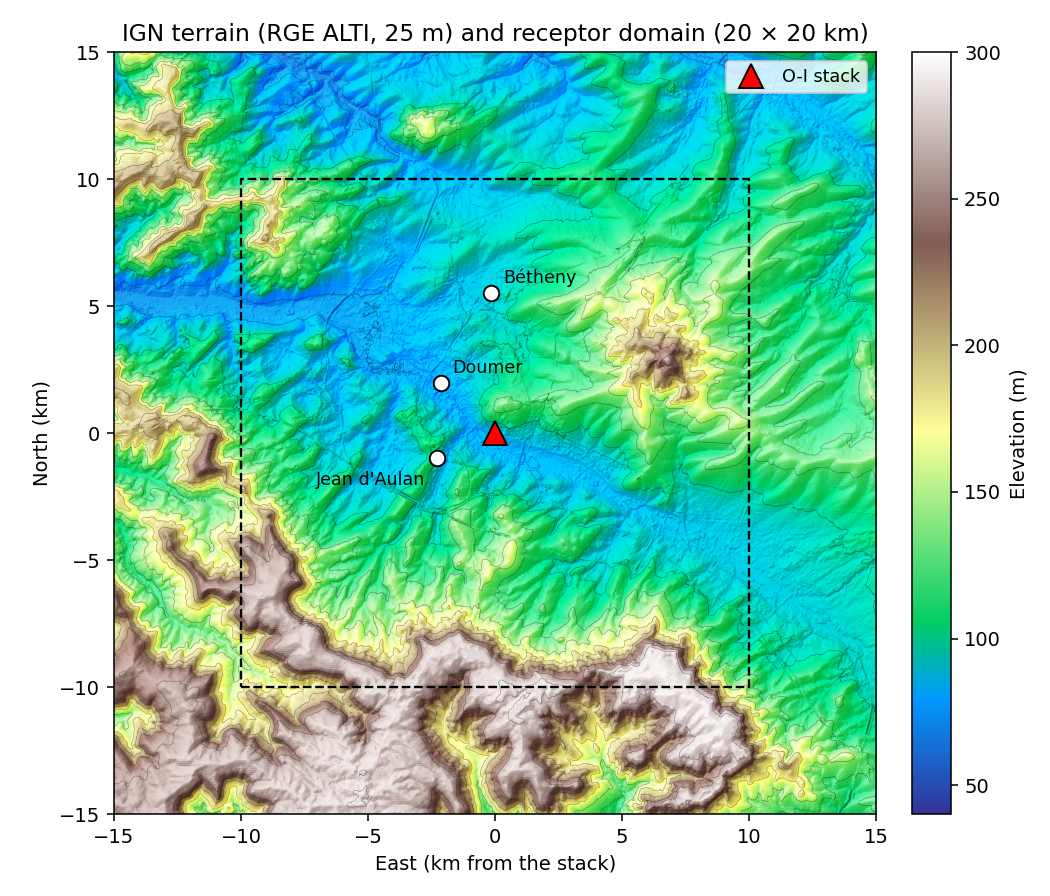
\includegraphics[width=0.62\textwidth]{relief_recepteurs_en.png}
\caption{Terrain around the plant and receptor domain. Mont de Berru (east) and the Montagne de Reims (south) rise
100 to 200~m above the plain.}
\end{figure}

\section{Method}
\textbf{Meteorology.} AERMET processes the Prunay data with the surface characteristics of the measurement site, as
the EPA requires for measured winds (farmland: \zz{} from 0.03~m in winter to 0.15~m in summer). The low-wind
u\textsuperscript{*} adjustment (ADJ\_U*) is enabled. 98 to 100~\% of hours are usable.

\textbf{Rural or urban.} AERMOD treats the nocturnal boundary layer differently in cities. The two EPA criteria
disagree here: the Auer (1978) land-use method within 3~km gives \emph{rural} (24~\% urban land), whereas population
density (about 3\,000 inhabitants/km², against a threshold of 750) gives \emph{urban}. Results are therefore given
as a range: rural option (reference) and urban option (population 182\,000, upper bound).

\textbf{Conversion to \NOd.} The OLM and ARM2 methods both give \NOd{}~=~0.9 × \NOx{} at every hour: measured ozone
(52~\ugm{} on average) is always in excess compared with the plant's \NOx.

\textbf{Comparison with measurements.} Three tests: averages by wind sector in 2024; a ``natural experiment''
2013–2025, which exploits the factor-of-4 variation in declared emissions (143 to 566~t/yr); and an hourly regression
of measured \NOx{} on the modelled contribution, with time-of-day and wind-speed effects.

\textbf{Simulated meteorology.} To test how representative Prunay is, WRF was run at 1~km for January and July 2024.
MMIF extracts the stack grid cell and prepares the AERMET input.

\section{Results for 2024}
\begin{table}[htbp]
\centering\small
\caption{Contribution of the glass plant in 2024 (buildings included).}
\begin{tabular}{lcc}
\toprule
Indicator & Rural (reference) & Urban (upper bound) \\
\midrule
Maximum annual mean (\NOx), 0.7~km north-east & 0.22~\ugm & 0.28~\ugm \\
Maximum hourly value (\NOx) & 49~\ugm{} (Mont de Berru) & 14~\ugm \\
Annual mean at the 3 stations (\NOd) & 0.03 to 0.05~\ugm & 0.05 to 0.13~\ugm \\
Share of measured \NOd{} at the stations & < 0.5~\% & 0.5 to 1.4~\% \\
\bottomrule
\end{tabular}
\end{table}

\begin{figure}[htbp]
\centering
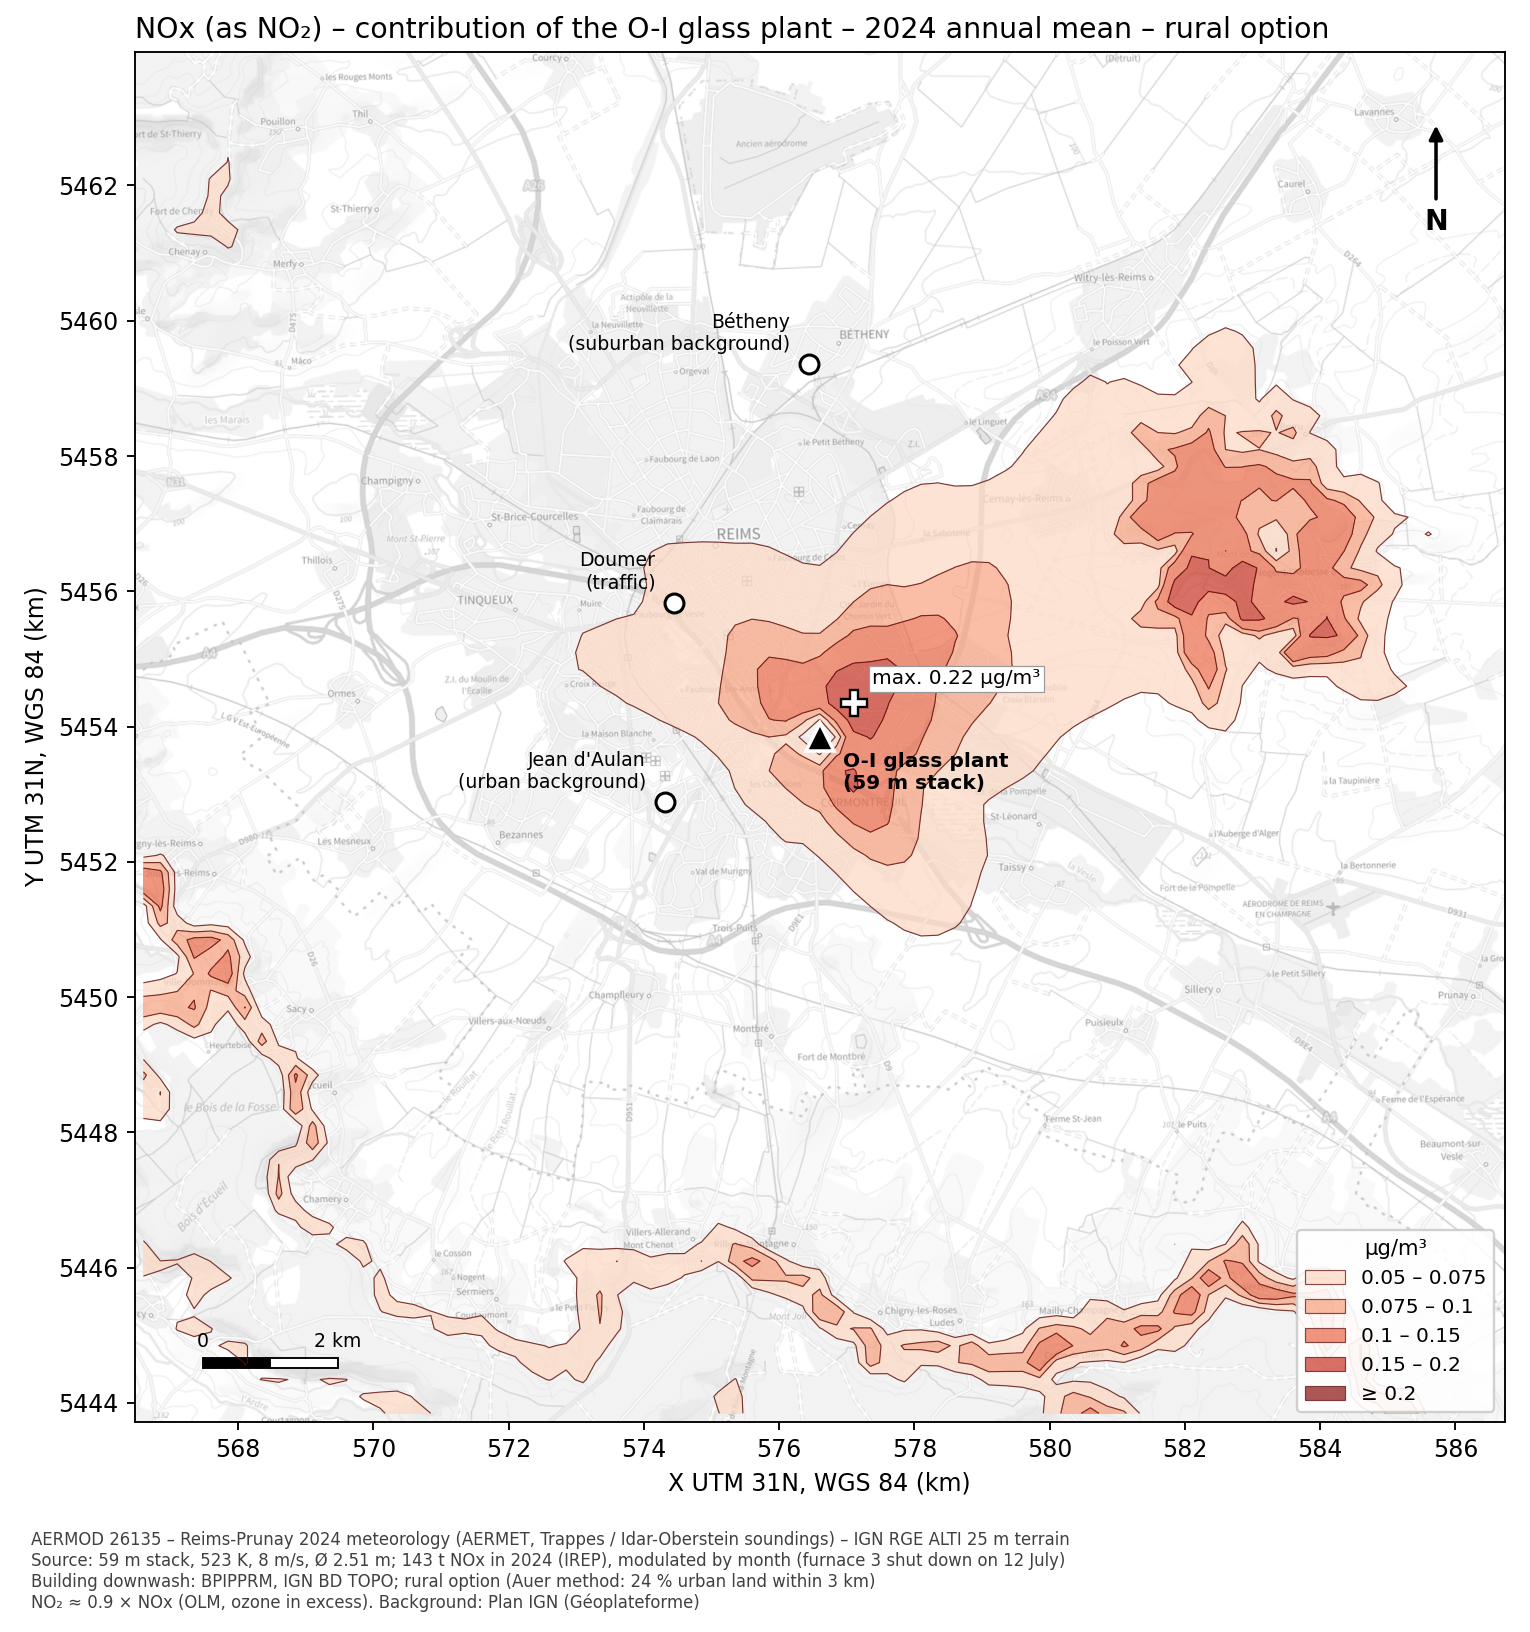
\includegraphics[width=0.49\textwidth]{aermod_rural_2024_annuel_en.png}\hfill
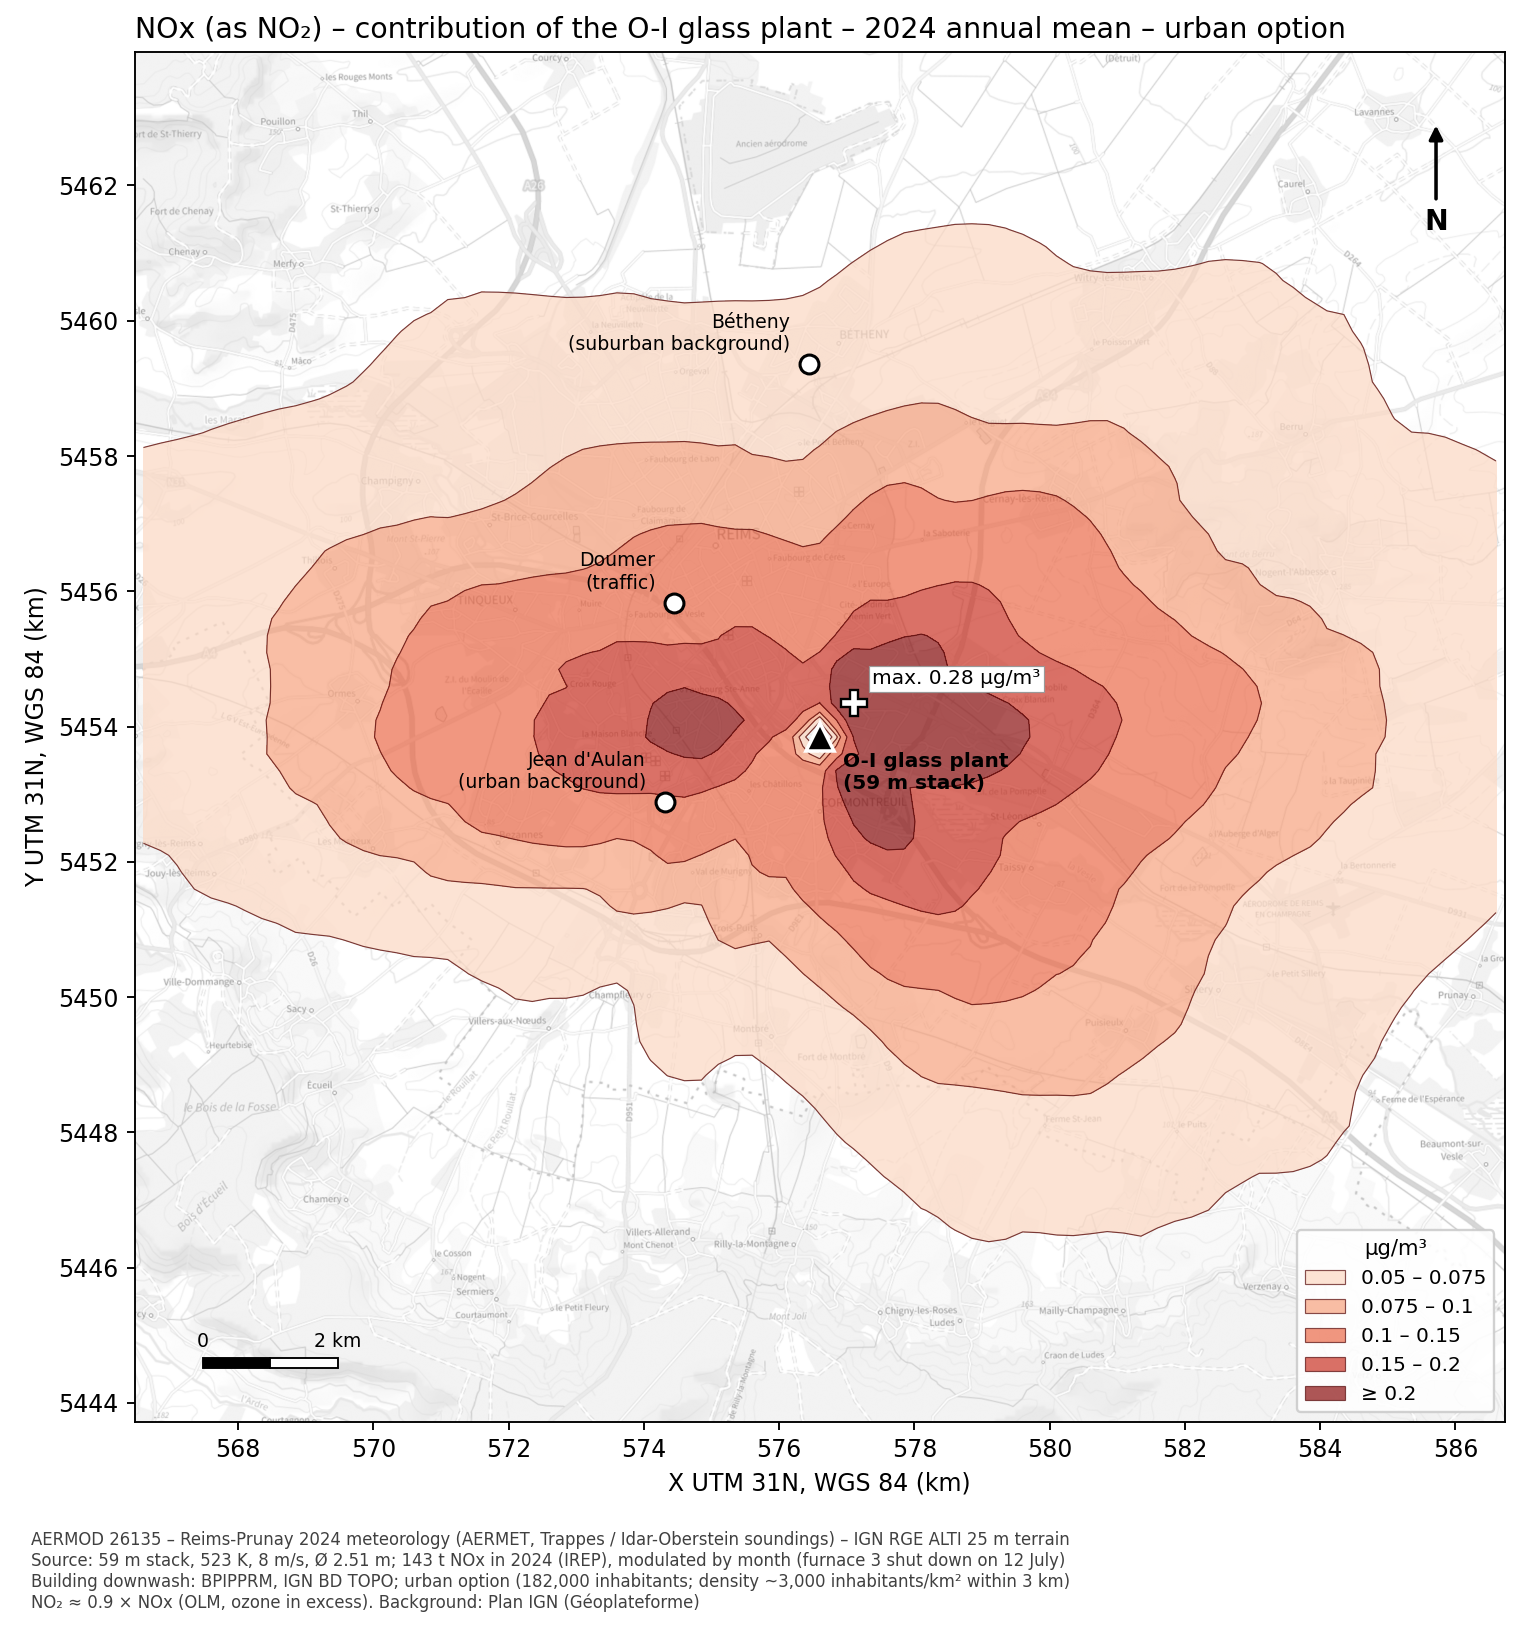
\includegraphics[width=0.49\textwidth]{aermod_reference_2024_annuel_en.png}
\caption{2024 annual mean contribution of the plant (\NOx), rural option (left) and urban option (right), with the
same classes. Nothing is coloured below 0.05~\ugm.}
\end{figure}

The plume travels mainly north-east, under the prevailing south-westerly winds. With the rural option it also
reaches the high ground 6–7~km away (Mont de Berru) and the slopes of the Montagne de Reims. The urban option gives a
wider, more symmetric footprint, with a westward lobe over Jean d'Aulan and Doumer. This is why it gives 2 to 4 times
more at the stations, although its maximum is hardly higher. Neither option is the more conservative everywhere: the
urban option gives more on the annual mean, the rural option more on the hourly maximum, because of the terrain
(Fig.~\ref{fig:max1h}).

\begin{figure}[htbp]
\centering
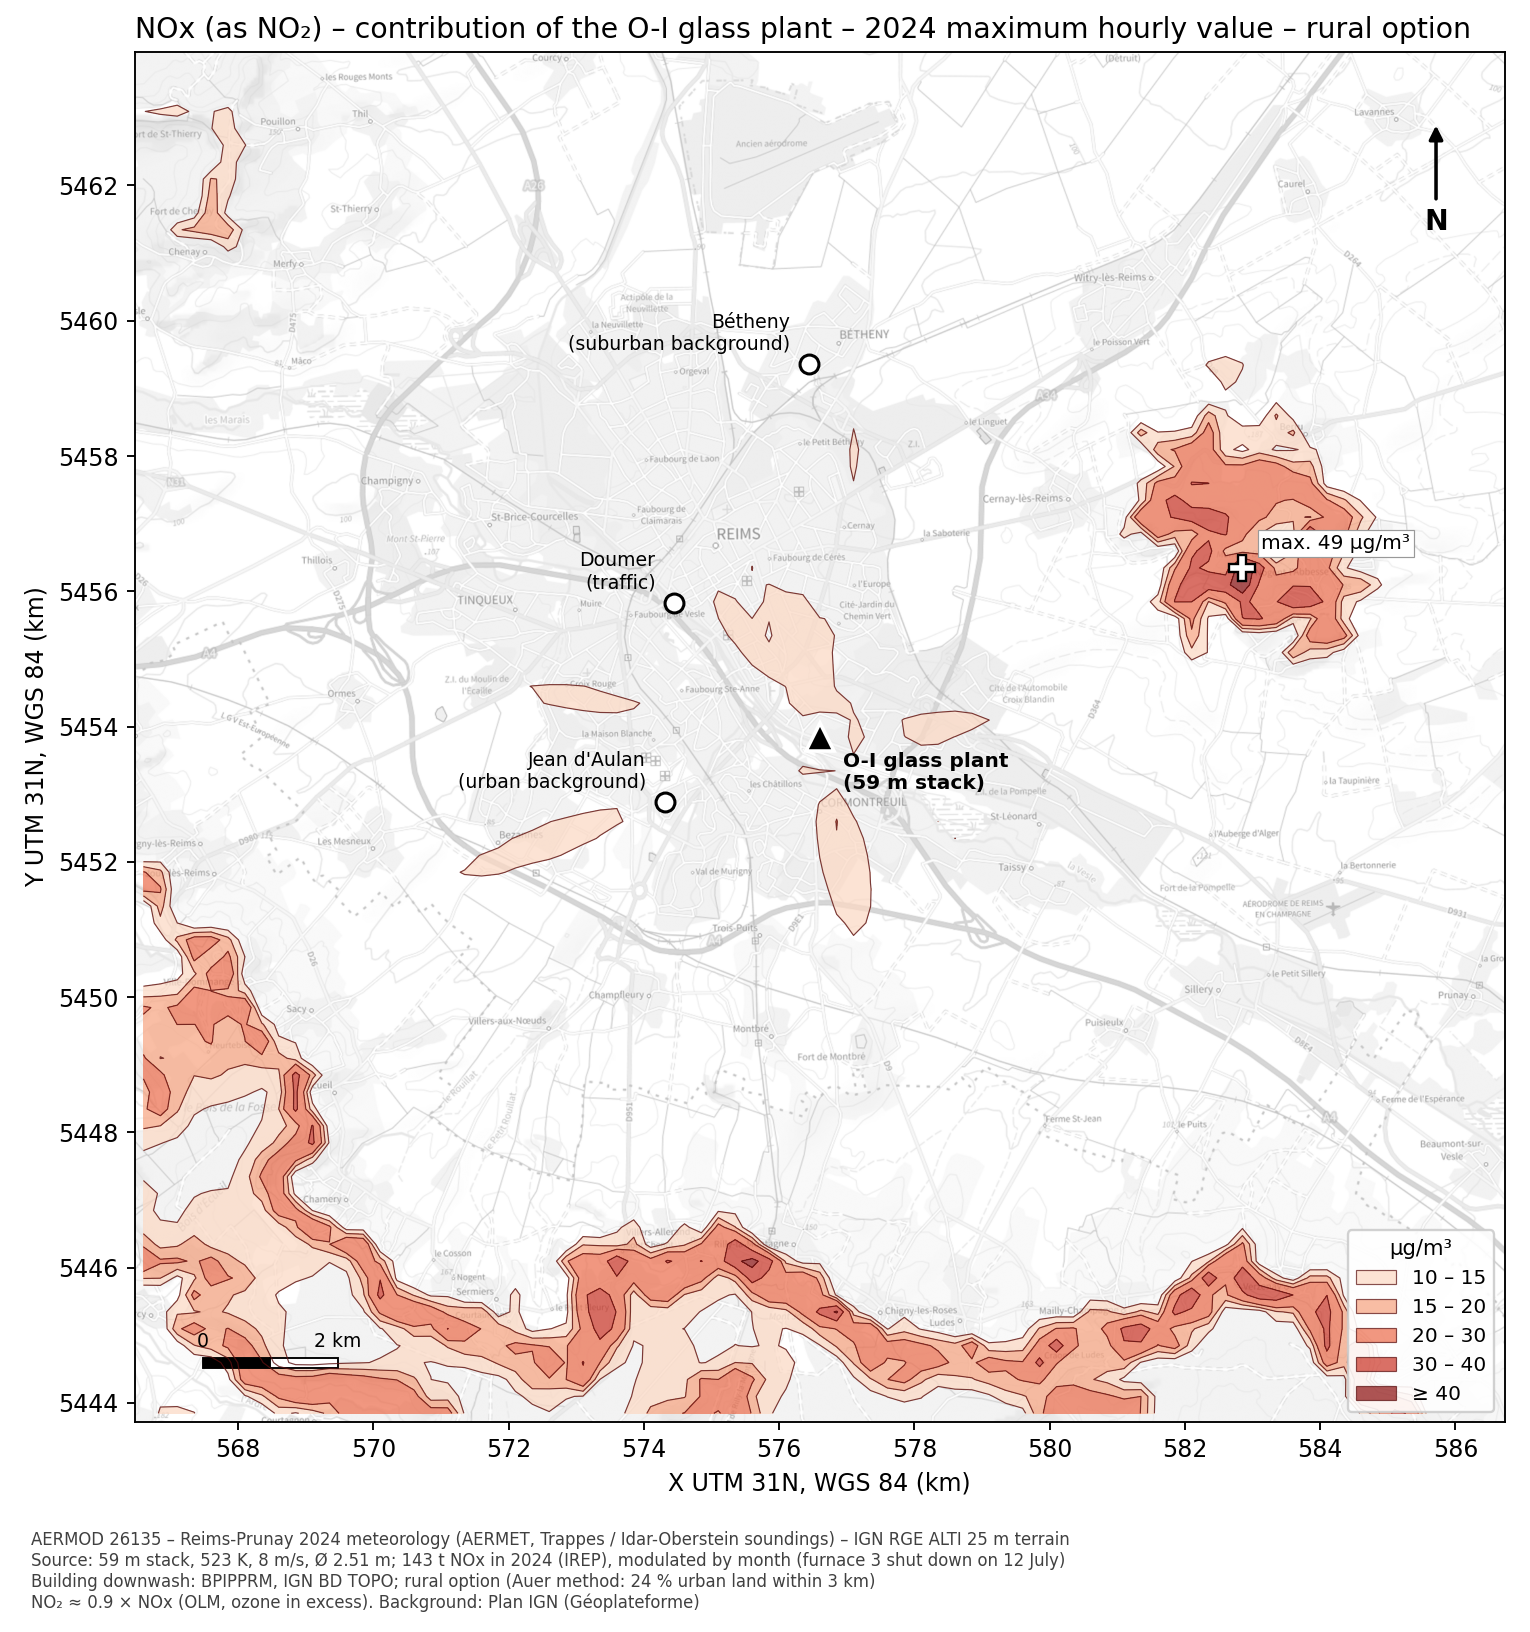
\includegraphics[width=0.49\textwidth]{aermod_rural_2024_max1h_en.png}\hfill
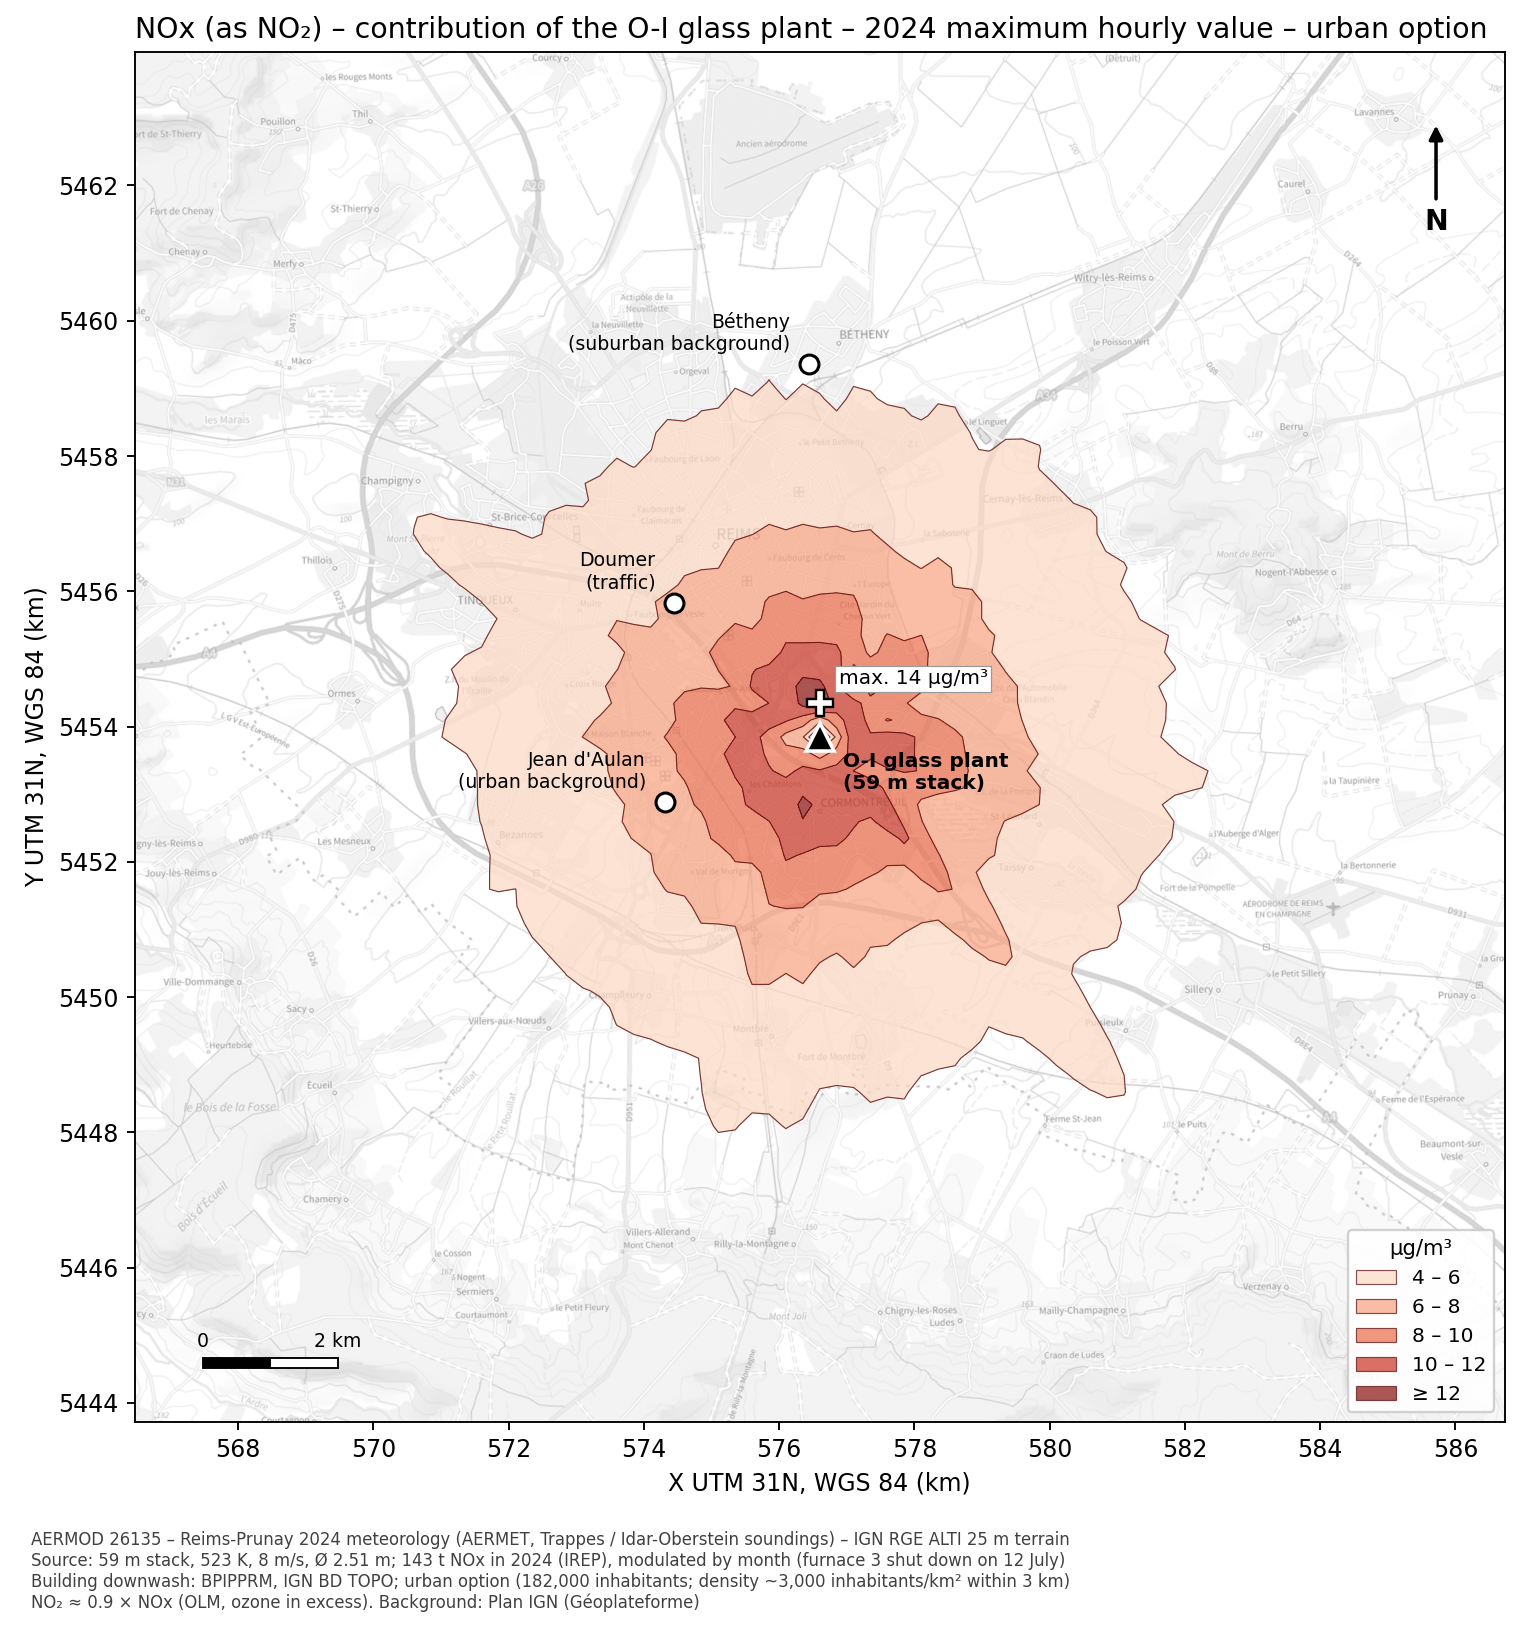
\includegraphics[width=0.49\textwidth]{aermod_reference_2024_max1h_en.png}
\caption{2024 maximum hourly contribution (\NOx), rural option (left, 49~\ugm{} on Mont de Berru) and urban option
(right, 14~\ugm). Each map has its own classes: compare the values, not the colours.}
\label{fig:max1h}
\end{figure}

\section{Comparison with measurements}
\textbf{By wind sector.} The model places the plant's influence in a narrow peak (±\,15°) in the direction of the
plant as seen from each station. Averaged over that sector, the modelled contribution is 0.3 to 0.5~\ugm{} of \NOd{}
with the rural option and 0.7 to 1.6~\ugm{} with the urban option, i.e.\ 2 to 11~\% of the \NOd{} measured in the
same sector. The measurements show no such peak: the variation of \NOd{} with wind direction (a factor of 2 to 3)
follows the weather situations. Cold, stable north-easterly winds give the highest \NOd{} at all three stations at
once, including where the plant does not lie in that direction (Fig.~\ref{fig:secteurs}).

\begin{figure}[htbp]
\centering
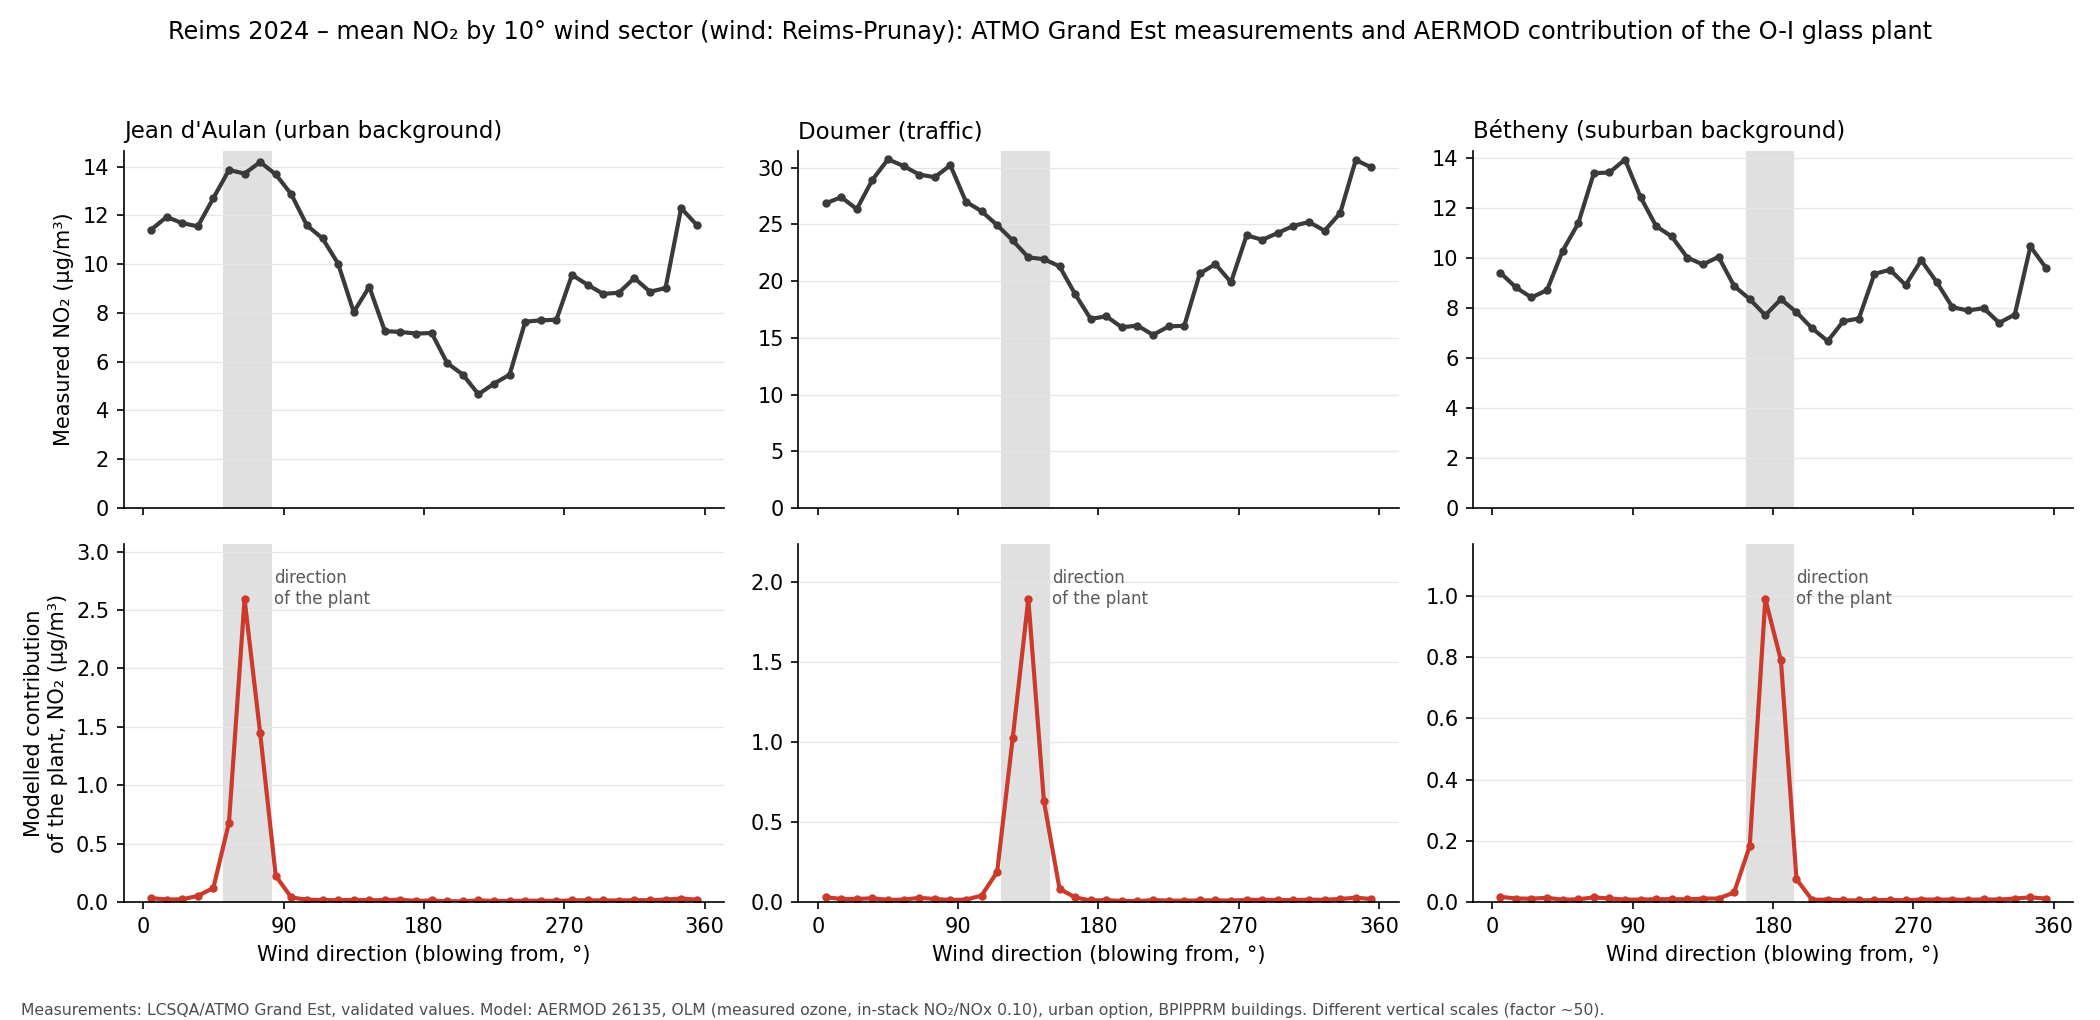
\includegraphics[width=\textwidth]{etape6_secteurs_no2_en.png}
\caption{Mean \NOd{} by 10° wind sector in 2024: measurements (top) and modelled contribution of the plant, urban
option (bottom; vertical scales differ by a factor of about 50). Grey band: direction of the plant.}
\label{fig:secteurs}
\end{figure}

\textbf{Natural experiment 2013–2025.} If the plant contributed noticeably, the \NOd{} excess when the wind blows
from the plant (relative to neighbouring sectors) would follow its annual emissions. We measure the slope of this
excess against emissions, relative to the slope predicted by AERMOD ($\beta = 1$ if the model is right, $\beta = 0$
if the plant has no visible effect). If the Prunay wind direction were exact, we would obtain
$\beta = -0.16 \pm 0.22$ for the urban option and $\beta = -0.08 \pm 0.65$ for the rural option (Fig.~\ref{fig:exp}).
However, the difference in direction between the Prunay wind and the WRF wind at the plant's grid cell has a robust
standard deviation of 26° in January and 38° in July. With a direction error of 20 to 40°, the urban option is
disfavoured by only 1.1 to 2.2 standard deviations, and the rural option remains compatible. The test indicates a
preference; it is not conclusive.

\begin{figure}[htbp]
\centering
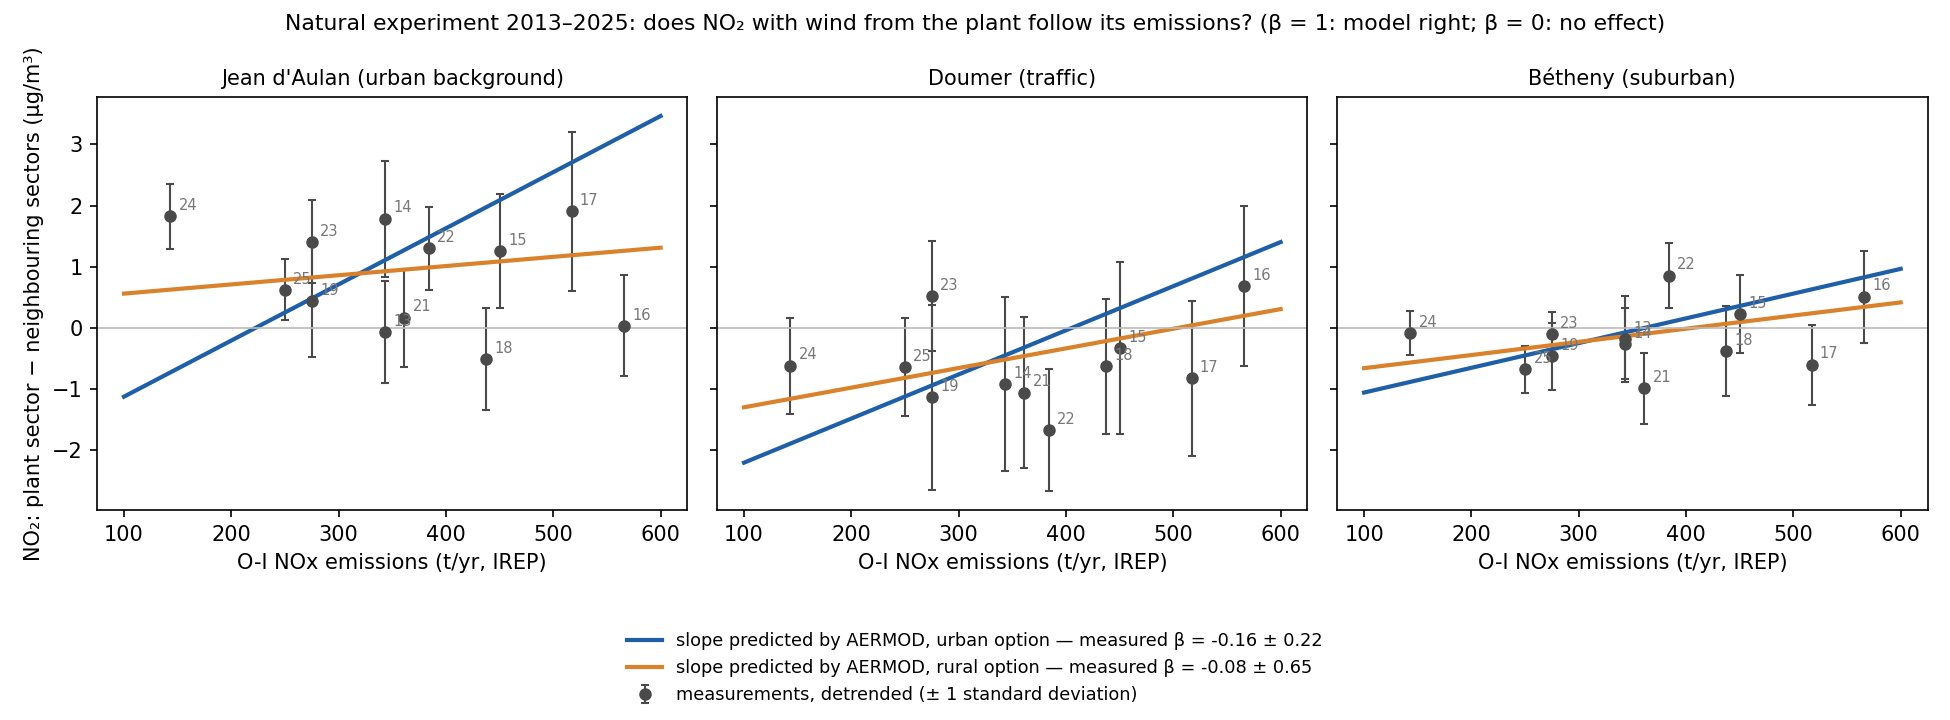
\includegraphics[width=\textwidth]{etape6_experience_naturelle_en.png}
\caption{\NOd{} excess when the wind blows from the plant versus O-I's annual emissions, 2013–2025, and slopes
predicted by AERMOD (wind direction assumed exact).}
\label{fig:exp}
\end{figure}

\textbf{Hour by hour.} Without controls, the rank correlation between measured \NOx{} and the modelled contribution is
$-0.3$ to $-0.4$ with the rural option and $+0.3$ to $+0.4$ with the urban option (January). The sign depends on the
option, not on the plant. In rural mode, the plume reaches the stations in brisk winds, when urban air is clean; in
urban mode, it reaches them in calm weather, when traffic \NOx{} builds up. Once time of day and wind speed are taken
into account, the slope $\beta$ cannot be measured: its standard errors range from 0.45 to 24 over 42 regressions
(7 cases, 3 stations, 2 months). The plant's signal (0.3 to 4.6~\ugm{} at the 99th hourly percentile) is lost in
hourly variations of 5 to 63~\ugm.

\textbf{Heat island of the plant.} Paine et al.\ (2016) justify the urban option near a large plant if it creates a
heat island of at least 8~K over a few hundred metres. On 32 cloud-free Landsat images, the plant has its own but
moderate thermal signature: +1.7~K on average within 300~m in winter, and no pixel above +8~K. On 9 ASTER night
images, it does not stand out from the urban fabric: +1.2~K on average, and no pixel above +4~K. The criterion is not
met, so the urban option is not justified by an effect specific to the plant.

\section{Meteorology simulated with WRF}
Prunay lies 7~km away, in open country. WRF was therefore run at 1~km resolution, and AERMOD was rerun with the
meteorology of the stack grid cell. According to the EPA (MMIF guidance, Sect.~3.3), the surface characteristics of
the model grid cell, as provided by MMIF, must then be used. The 1~km cell is classified as ``urban'', with
\zz{}~=~0.8~m. However, Corine shows that the kilometre around the stack is half open or wooded: 32~\% discontinuous
urban fabric, 14~\% industrial areas, 19~\% crops, 17~\% sport and leisure areas, 12~\% forest and 7~\% vineyards. A
variant with \zz{}~=~0.25~m estimated from these classes was therefore added.

\begin{table}[htbp]
\centering\small
\caption{Monthly mean contribution (\NOx, \ugm) at Jean d'Aulan / Doumer / Bétheny.}
\begin{tabular}{lcc}
\toprule
Meteorology, option & January 2024 & July 2024 \\
\midrule
Prunay, rural (reference) & 0.025 / 0.029 / 0.044 & 0.057 / 0.073 / 0.024 \\
Prunay, urban & 0.195 / 0.115 / 0.078 & 0.142 / 0.130 / 0.055 \\
WRF, MMIF surface (\zz{} 0.8~m), rural & 0.115 / 0.164 / 0.054 & 0.050 / 0.042 / 0.019 \\
WRF, MMIF surface, urban & 0.222 / 0.237 / 0.077 & 0.106 / 0.127 / 0.035 \\
WRF, \zz{} 0.25~m, rural & 0.058 / 0.078 / 0.055 & 0.054 / 0.048 / 0.018 \\
WRF, \zz{} 0.25~m, urban & 0.183 / 0.255 / 0.085 & 0.109 / 0.144 / 0.038 \\
\bottomrule
\end{tabular}
\end{table}

\begin{itemize}
\item \textbf{In winter}, roughness is everything. With \zz{}~=~0.8~m, WRF's mechanical turbulence brings the plume
down near the source: a monthly maximum of 1.8~\ugm{} at 0.4~km, and × 1.2 to × 5.7 at the stations compared with
Prunay. With \zz{}~=~0.25~m, the ratio is × 1.2 to × 2.7.
\item \textbf{In summer}, convection dominates (mixed layer of 700 to 1\,000~m by day): WRF gives back the Prunay
values at the stations (× 0.6 to × 1).
\item \textbf{High roughness.} Tests with \zz{}~=~1, 1.5 and 2~m give at most 0.17~\ugm{} at the stations with the
rural option. Above \zz{} $\approx$ 1.4~m, AERMET no longer accepts the 10~m wind as reference wind: it must be
measured at least 7\,\zz{} above ground (AERMET guide), and the response becomes irregular. With a wind measured
only at 10~m, AERMOD therefore cannot handle city-centre roughness.
\end{itemize}
In all cases, the contribution at the stations stays at or below 0.26~\ugm{} over the month: simulated meteorology
does not change the order of magnitude.

\begin{figure}[htbp]
\centering
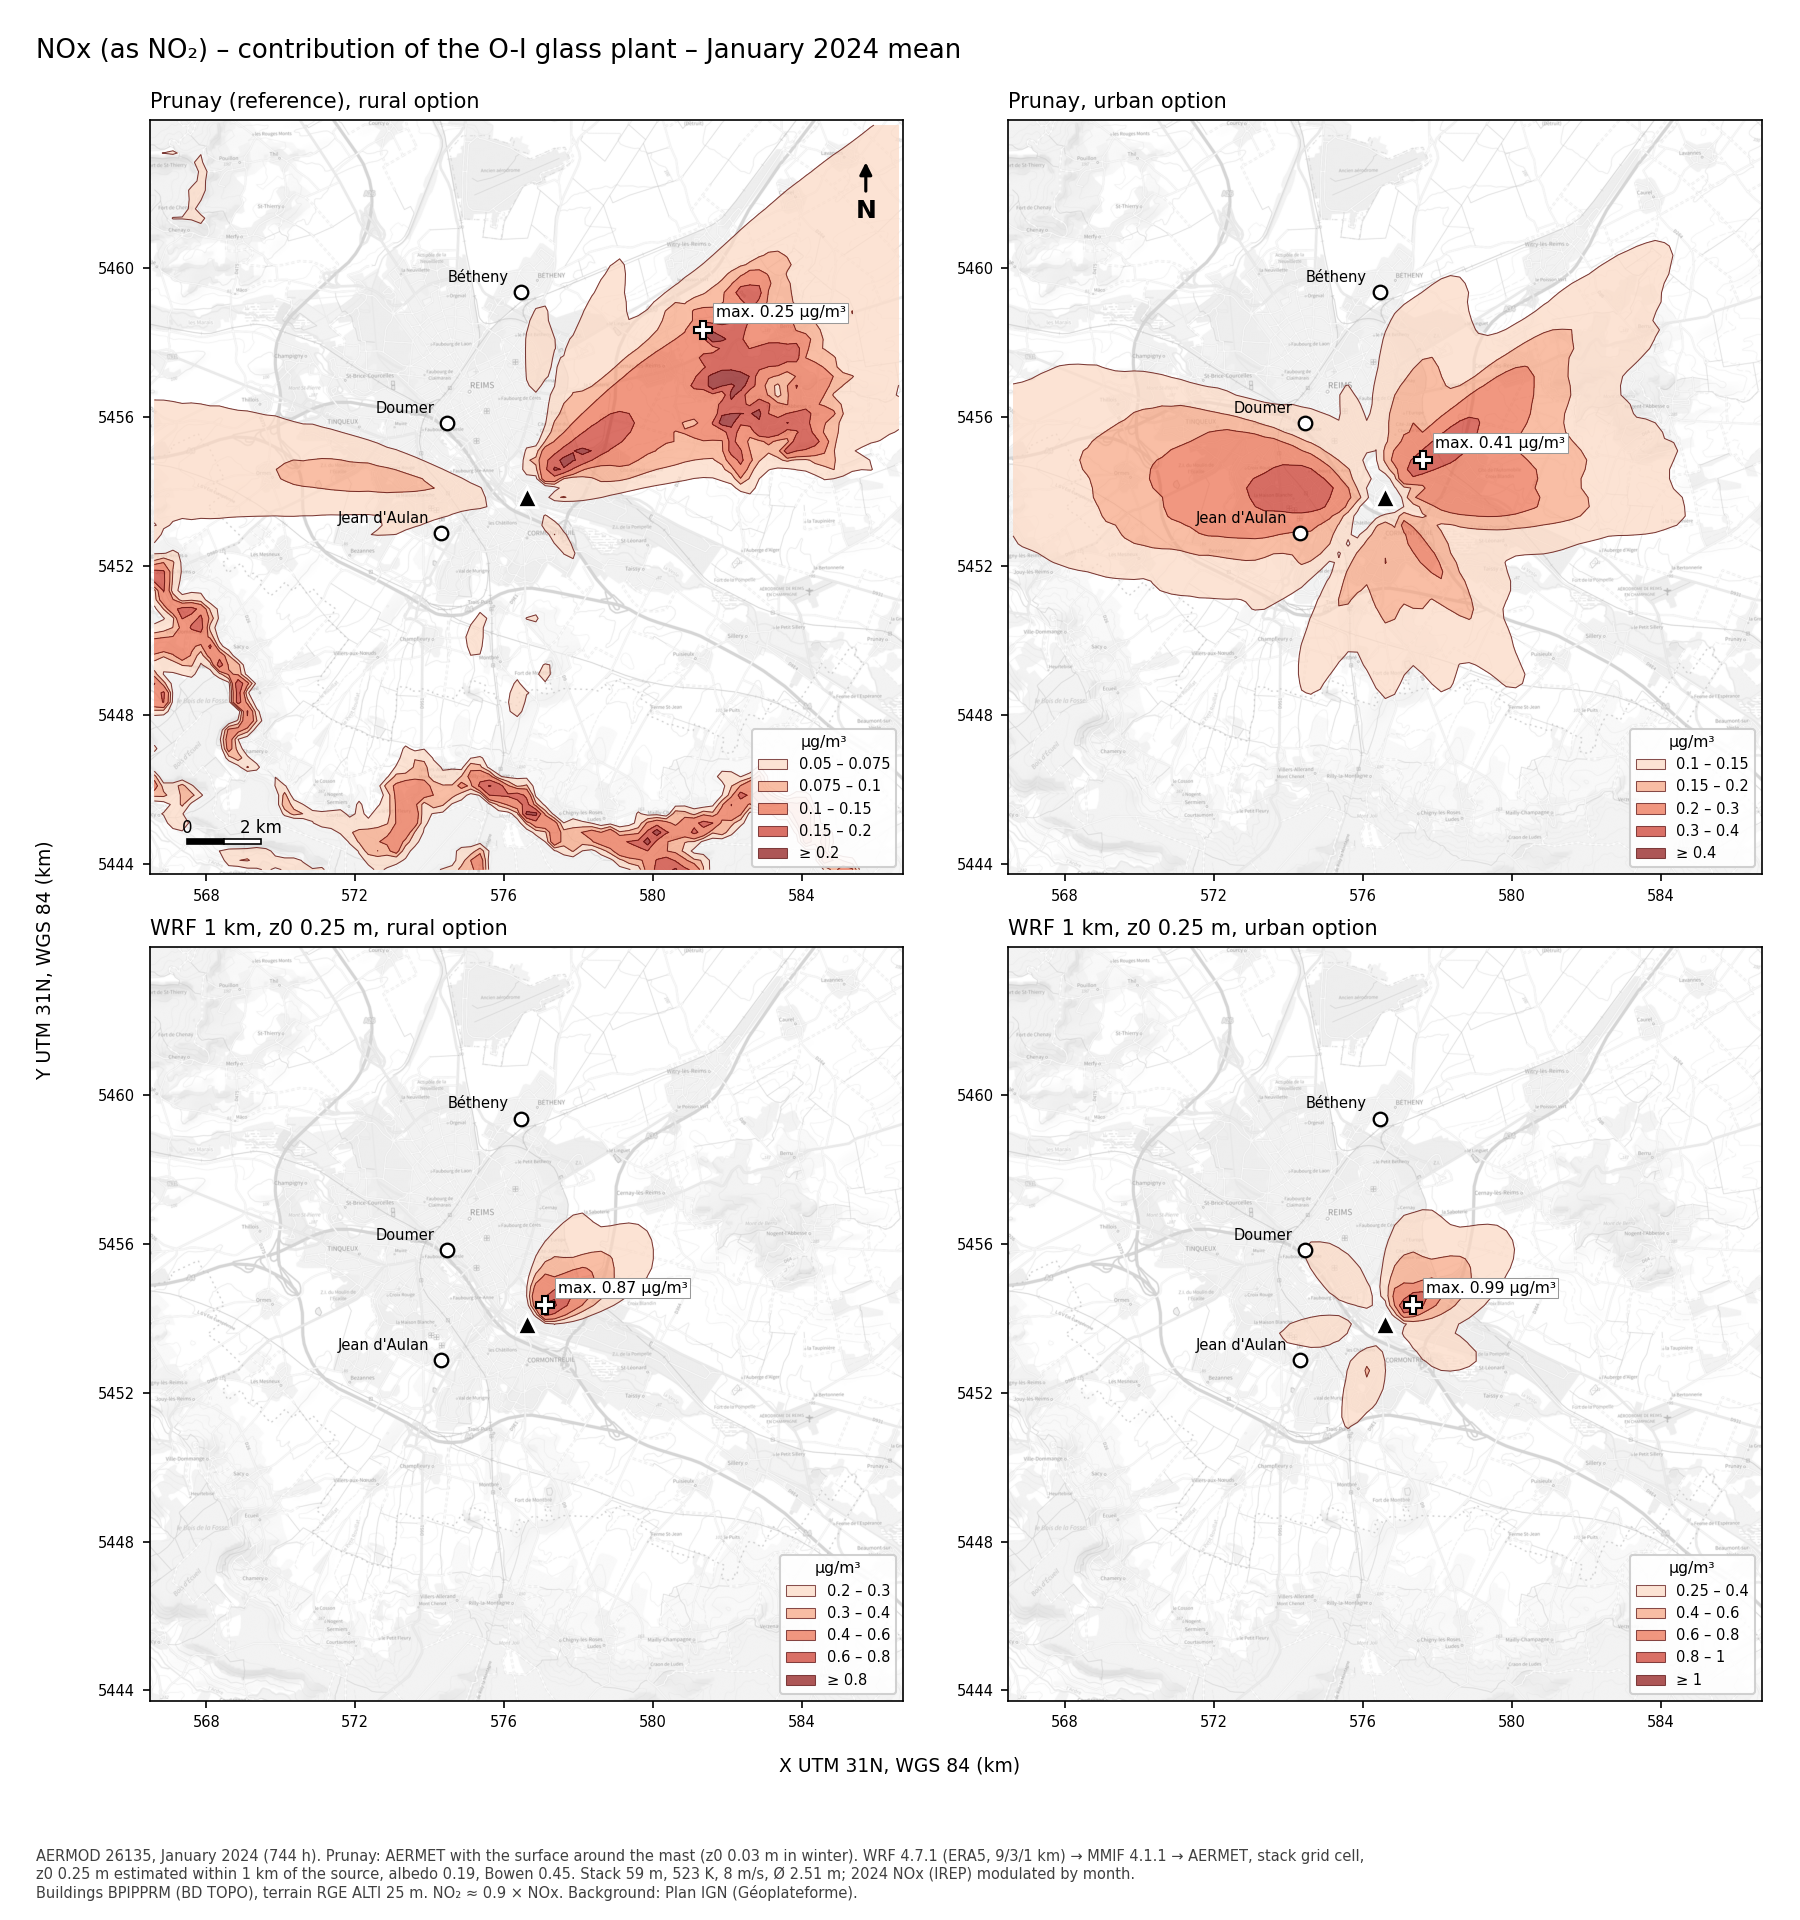
\includegraphics[width=0.70\textwidth]{etape8_janvier_moyenne_en.png}
\caption{January 2024 mean (\NOx): Prunay (top) and WRF with \zz{}~=~0.25~m (bottom), rural and urban options. Each
map has its own classes.}
\end{figure}

\section{Other sources of uncertainty}
\begin{table}[htbp]
\centering\small
\caption{Effect of each assumption, tested one at a time.}
\begin{tabularx}{\textwidth}{lY}
\toprule
Assumption & Effect \\
\midrule
Rural or urban & dominant factor: stations × 2 to × 4.6; hourly maximum $-72$~\% \\
Simulated meteorology (WRF, 1~km) & stations × 1.2 to × 5.7 in winter, × 0.6 to × 1 in summer; always $\leq$ 0.26~\ugm{} \\
Prunay roughness raised to 0.25~m & +18 to 20~\% at the stations \\
Flue-gas temperature ± 50~°C & ± 10 to 20~\% \\
Declared emissions & proportional \\
Diameter, location, buildings, hourly emission profile & < 7~\% \\
Measured radiation instead of cloud cover & +8 to 12~\% on the annual maximum, 0 to +6~\% at the stations \\
Fog (112~h in 2024) & rural contribution close to zero during fog \\
Morning fumigation (AERSCREEN) & 6.5~\ugm{} over 1~h at 9.3~km, below the other hourly maxima \\
\bottomrule
\end{tabularx}
\end{table}

\textbf{Radiation.} AERMET estimates solar radiation from cloud cover (Kasten and Czeplak, 1980). Compared with the
global radiation measured at Prunay, it is correct on average ($-9$~\%, $r = 0.86$) but underestimates overcast days by
32~\%. Recomputing cloud cover from the measured radiation changes the results little.

\textbf{Fog.} During the 112 hours of fog in 2024, AERMET describes a stable, shallow boundary layer (mixed layer of
67~m). Measured \NOx{} is then 2 to 3.5 times higher, because traffic emissions accumulate. The plume, being higher,
does not reach the ground with the rural option. A minor anomaly: AERMET sees 14~\% of these hours as clear sky.

\textbf{Fumigation.} In the morning, when the inversion breaks up, a plume that stayed aloft can be brought down to
the ground at once. AERMOD does not simulate this. AERSCREEN, the EPA screening tool (method of Turner, 1970), places
this fumigation at 9.3~km. By then the plume has had time to spread, and the concentration does not exceed
6.5~\ugm.

\section{Health aspects}
For the 173 sensitive establishments within 4~km (BD TOPO), the plant's contribution to \NOd{} is at most 0.10 to
0.19~\ugm{} as an annual mean, 2.1~\ugm{} over 24~h and 11~\ugm{} over 1~h. Taking the less favourable of the two
options, the plant's hazard quotient is at most 0.02 for the annual mean (WHO guideline, 10~\ugm) and 0.06 for 1~h
(200~\ugm). Total exposure, about 9.5~\ugm, is dominated by the urban background.

\section{Limitations and outlook}
\begin{itemize}
\item \textbf{Emissions}: only the declared annual total is known, distributed by month according to production. Real
hourly flows and degraded operation (backup stacks) are not represented.
\item \textbf{Stack parameters}: values prescribed by the permit (minimum velocity, nominal flow), not measured.
\item \textbf{Rural or urban}: the question remains open. Measurements disfavour the urban option without ruling it
out, and the EPA criteria disagree.
\item \textbf{Meteorology}: Prunay is 7~km away, and WRF was run for only two months. A full year would require about
18 days of computing.
\item \textbf{Validation}: the stations, 2.5–5.5~km away, cannot settle the question. Neither can passive tubes: the
plant's contribution over 14 days (0.1 to 0.8~\ugm{} at 0.5–1~km) is well below their uncertainty (± 3 to
4~\ugm). Validation would require hourly \NOx{} and \SOd{} analysers and an anemometer 0.5–1~km north-east of the
plant, together with the stack's actual hourly emissions.
\end{itemize}

\section{Conclusions}
\begin{enumerate}
\item The glass plant contributes less than 0.5~\% (rural option) to 1.4~\% (urban option) of the mean \NOd{}
measured at the Reims stations. Urban \NOd{} is dominated by traffic and by stagnant weather situations.
\item The network does not see the plant directly. Thirteen years of measurements disfavour the urban option without
ruling it out.
\item The rural/urban choice is the main source of uncertainty. No other factor tested changes the order of
magnitude.
\item The plant matters only close by (within 1~km to the north-east) and, at some hours, on the high ground. The
health risk associated with its contribution is low.
\end{enumerate}

\section{Data and code}\label{sec:repro}
Repository: \url{https://github.com/Mahamat-A/aermod-reims-verrerie}, archived on Zenodo
(\url{https://doi.org/10.5281/zenodo.24559574}) (AERMET, AERMAP, AERMOD, MMIF and AERSCREEN inputs, Python scripts,
figures in French and English, detailed step reports in French). Software: AERMOD 26135, AERMET, AERMAP 24142, BPIPPRM, AERSCREEN 21112
(EPA), MMIF 4.1.1, WRF 4.7.1. Data remain subject to their providers' terms (NOAA, Météo-France, IGN, LCSQA, EEA,
Copernicus).

\section*{References}
\small
\begin{description}[leftmargin=0pt,labelindent=0pt,itemsep=1pt,font=\normalfont]
\item Auer, A.\,H. (1978). Correlation of land use and cover with meteorological anomalies. \textit{Journal of
Applied Meteorology}, 17, 636–643.
\item Cimorelli, A.\,J. et al. (2005). AERMOD: A dispersion model for industrial source applications. Part I:
General model formulation and boundary layer characterization. \textit{Journal of Applied Meteorology}, 44, 682–693.
\item Hersbach, H. et al. (2020). The ERA5 global reanalysis. \textit{Quarterly Journal of the Royal Meteorological
Society}, 146, 1999–2049.
\item Kasten, F. and Czeplak, G. (1980). Solar and terrestrial radiation dependent on the amount and type of cloud.
\textit{Solar Energy}, 24, 177–189.
\item Paine, R., Warren, L.\,L. and Moore, G.\,E. (2016). Source characterization refinements for routine modeling
applications. \textit{Atmospheric Environment}, 129, 55–67. doi:10.1016/j.atmosenv.2016.01.003.
\item Skamarock, W.\,C. et al. (2019). \textit{A description of the Advanced Research WRF Model Version 4}. NCAR
Technical Note NCAR/TN-556+STR.
\item Turner, D.\,B. (1970). \textit{Workbook of Atmospheric Dispersion Estimates}. US Public Health Service,
publication 999-AP-26.
\item U.S. EPA (2021). \textit{AERSCREEN User's Guide}. EPA-454/B-21-005.
\item U.S. EPA (2024). \textit{Guidance on the Use of the Mesoscale Model Interface Program (MMIF) for AERMOD
Applications}. EPA-454/B-24-005.
\item U.S. EPA (2026). \textit{User's Guide for the AMS/EPA Regulatory Model (AERMOD)}. EPA-454/B-26-001.
\item U.S. EPA (2026). \textit{User's Guide for the AERMOD Meteorological Preprocessor (AERMET)}. EPA-454/B-26-005.
\end{description}

\end{document}
